\documentclass[11pt,]{article}
\usepackage[margin=1in]{geometry}
\newcommand*{\authorfont}{\fontfamily{phv}\selectfont}
\usepackage[]{mathpazo}

\usepackage{amssymb,amsmath}
\usepackage{xcolor}

%TIKZ and Flow chart material
\usepackage{tikz}
\usetikzlibrary{shapes.geometric, arrows}
\tikzstyle{startstop} = [rectangle, rounded corners, minimum width=3cm, minimum height=1cm,text centered, draw=black, fill=red!30]
\tikzstyle{io} = [trapezium, trapezium left angle=70, trapezium right angle=110, minimum width=3cm, minimum height=1cm, text centered, draw=black,fill=white]
\tikzstyle{process} = [rectangle, minimum width=3cm, minimum height=1cm, text centered, draw=black, fill=white]
\tikzstyle{decision} = [diamond, minimum width=3cm, minimum height=1cm, text centered, draw=black, fill=white]
\tikzstyle{smalldecision} = [diamond, minimum width=1cm, minimum height=1cm, text centered, draw=black, fill=white]
\tikzstyle{arrow} = [thick,->,>=stealth]
\tikzstyle{line} = [thick,-]
\tikzstyle{dot} = [circle,inner sep=0.5pt,draw=black, fill=black]


%\tikzstyle{startstop} = [rectangle, rounded corners, minimum width=3cm, minimum height=1cm,text centered, %draw=black, fill=red!30]
%\tikzstyle{io} = [trapezium, trapezium left angle=70, trapezium right angle=110, minimum width=3cm, %minimum height=1cm, text centered, draw=black,fill=white]
%\tikzstyle{process} = [rectangle, minimum width=3cm, minimum height=1cm, text centered, draw=black, %fill=white]
%\tikzstyle{decision} = [diamond, minimum width=3cm, minimum height=1cm, text centered, draw=black, %fill=green!30]
%\tikzstyle{arrow} = [thick,->,>=stealth]




\usepackage{abstract}
\renewcommand{\abstractname}{}    % clear the title
\renewcommand{\absnamepos}{empty} % originally center
\newcommand{\blankline}{\quad\pagebreak[2]}

\providecommand{\tightlist}{%
  \setlength{\itemsep}{0pt}\setlength{\parskip}{0pt}}
\usepackage{longtable,booktabs}

\usepackage{parskip}
\usepackage{titlesec}
\titlespacing\section{0pt}{12pt plus 4pt minus 2pt}{6pt plus 2pt minus 2pt}
\titlespacing\subsection{0pt}{12pt plus 4pt minus 2pt}{6pt plus 2pt minus 2pt}

\titleformat*{\subsubsection}{\normalsize\itshape}

\usepackage{titling}
\setlength{\droptitle}{-.25cm}

%\setlength{\parindent}{0pt}
%\setlength{\parskip}{6pt plus 2pt minus 1pt}
%\setlength{\emergencystretch}{3em}  % prevent overfull lines

\usepackage[T1]{fontenc}
\usepackage[utf8]{inputenc}

\usepackage{fancyhdr}
\pagestyle{fancy}
\usepackage{lastpage}
\renewcommand{\headrulewidth}{0.3pt}
\renewcommand{\footrulewidth}{0.0pt}
%\lhead{\footnotesize Supplemental Problem Set }
\lhead{\footnotesize BUEC 311: Supplemental Problem Set, Graphing and
Manipulating Demand and Supply}
\rhead{\footnotesize \today}
\lfoot{\small \copyright }
\cfoot{}
\rfoot{\small \thepage/\pageref*{LastPage}}

\fancypagestyle{firststyle}
{
\renewcommand{\headrulewidth}{0pt}%
   \fancyhf{}
   \fancyfoot[C]{\thepage/\pageref*{LastPage}}
}

%\def\labelitemi{--}
%\usepackage{enumitem}
%\setitemize[0]{leftmargin=25pt}
%\setenumerate[0]{leftmargin=25pt}




\makeatletter
\@ifpackageloaded{hyperref}{}{%
\ifxetex
  \usepackage[setpagesize=false, % page size defined by xetex
              unicode=false, % unicode breaks when used with xetex
              xetex]{hyperref}
\else
  \usepackage[unicode=true]{hyperref}
\fi
}
\@ifpackageloaded{color}{
    \PassOptionsToPackage{usenames,dvipsnames}{color}
}{%
    \usepackage[usenames,dvipsnames]{color}
}
\makeatother
\hypersetup{breaklinks=true,
            bookmarks=true,
            pdfauthor={},
             pdfkeywords = {},
            pdftitle={Supplemental Problem Set: Graphing and
Manipulating Demand and Supply},
            colorlinks=true,
            citecolor=blue,
            urlcolor=blue,
            linkcolor=magenta,
            pdfborder={0 0 0}}
\urlstyle{same}  % don't use monospace font for urls


\setcounter{secnumdepth}{0}


%



\usepackage{setspace}

\title{\vspace{-1.5cm}\Large{BUEC 311: Business Economics, Organization
and Management}\medskip\\\Large{Supplemental Problem Set}
\medskip\\\Large{Graphing and Manipulating Demand and Supply}
}
\date{\vspace{-.75cm}\Large{\today}}

\definecolor{light-gray}{gray}{0.8}


\begin{document}

\vspace{-5cm}\maketitle
 \tikz [remember picture,overlay]
    %\node[yshift=-1.65cm,xshift=0cm] at (current page.north)
    %\node[yshift=-1.65cm,xshift=0cm] at (current page.north)
        %or: (current page.center)
        \node[yshift=-1cm,xshift=6.5cm] at (current page.north west)
        %{
\includegraphics[width=3in]{UA-ASB-COLOUR.png}};
        {
\includegraphics[width=.5\paperwidth]{../images/UA-ASB-COLOUR.png}};
\vspace{-.75cm}		
		\thispagestyle{firststyle}



This set will supplement some discussion of supply and demand curves in
this week's classes.

\begin{enumerate}
\def\labelenumi{\arabic{enumi}.}
\tightlist
\item
  First key task in a lot of this week will be inverting demand curves.
  Generally, demand curves are stated as quantity as a function of
  price, for example \(Q=10-2p\), while they are graphed as price as a
  function of quantity (the inverse demand).
\end{enumerate}

Step 1 before graphing anything is to make sure we're using the RIGHT
expression to match the graph we're trying to draw. In the case of
supply and demand, we always want to draw p on the vertical axis, as a
function of q on the horizonal axis:

\begin{center}
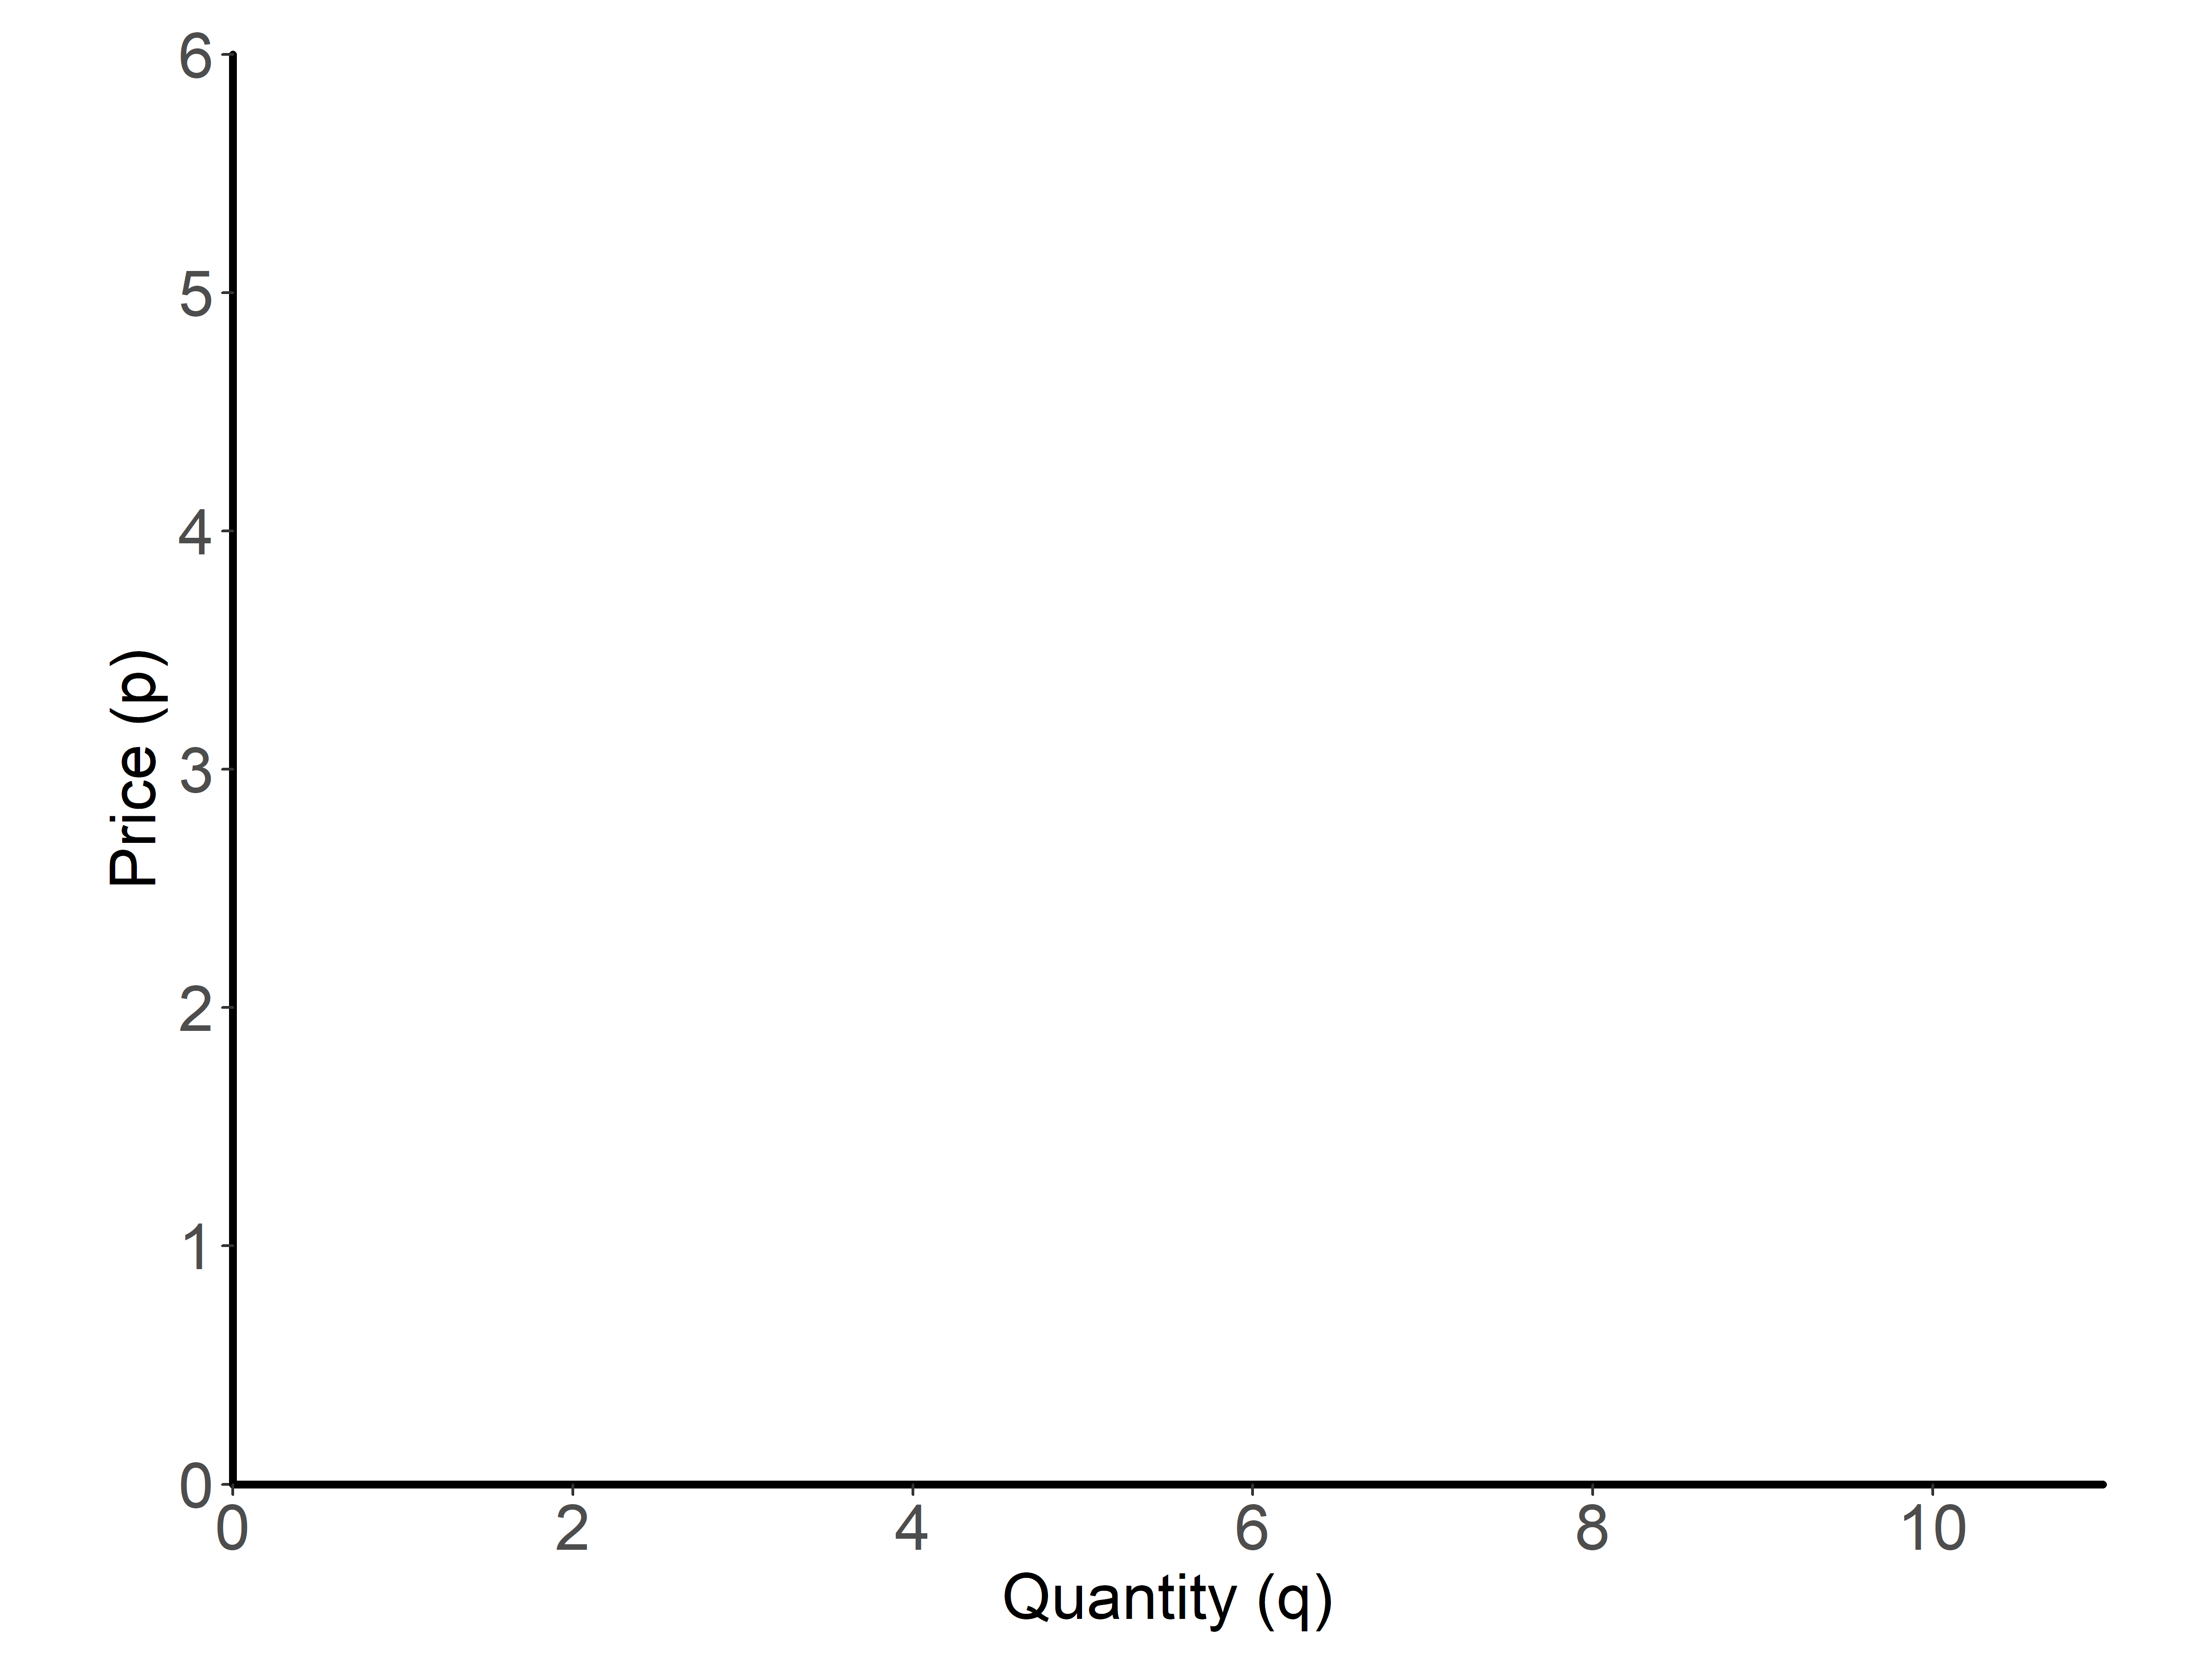
\includegraphics[width=0.65\textwidth]{../images/eq_blank.png}
\end{center}

So, we need to convert \(Q=10-2p\) into an equation with p as a function
of Q.

\begin{align*}
  Q&=10-2p\\
  \frac{Q}{2}&=5-p\,\text{, after dividing both sides by 2}\\
  p&=5-\frac{Q}{2}\,\text{, after rearranging terms}\\
\end{align*}

And now we have a p as a function of Q that we can graph:

\begin{center}
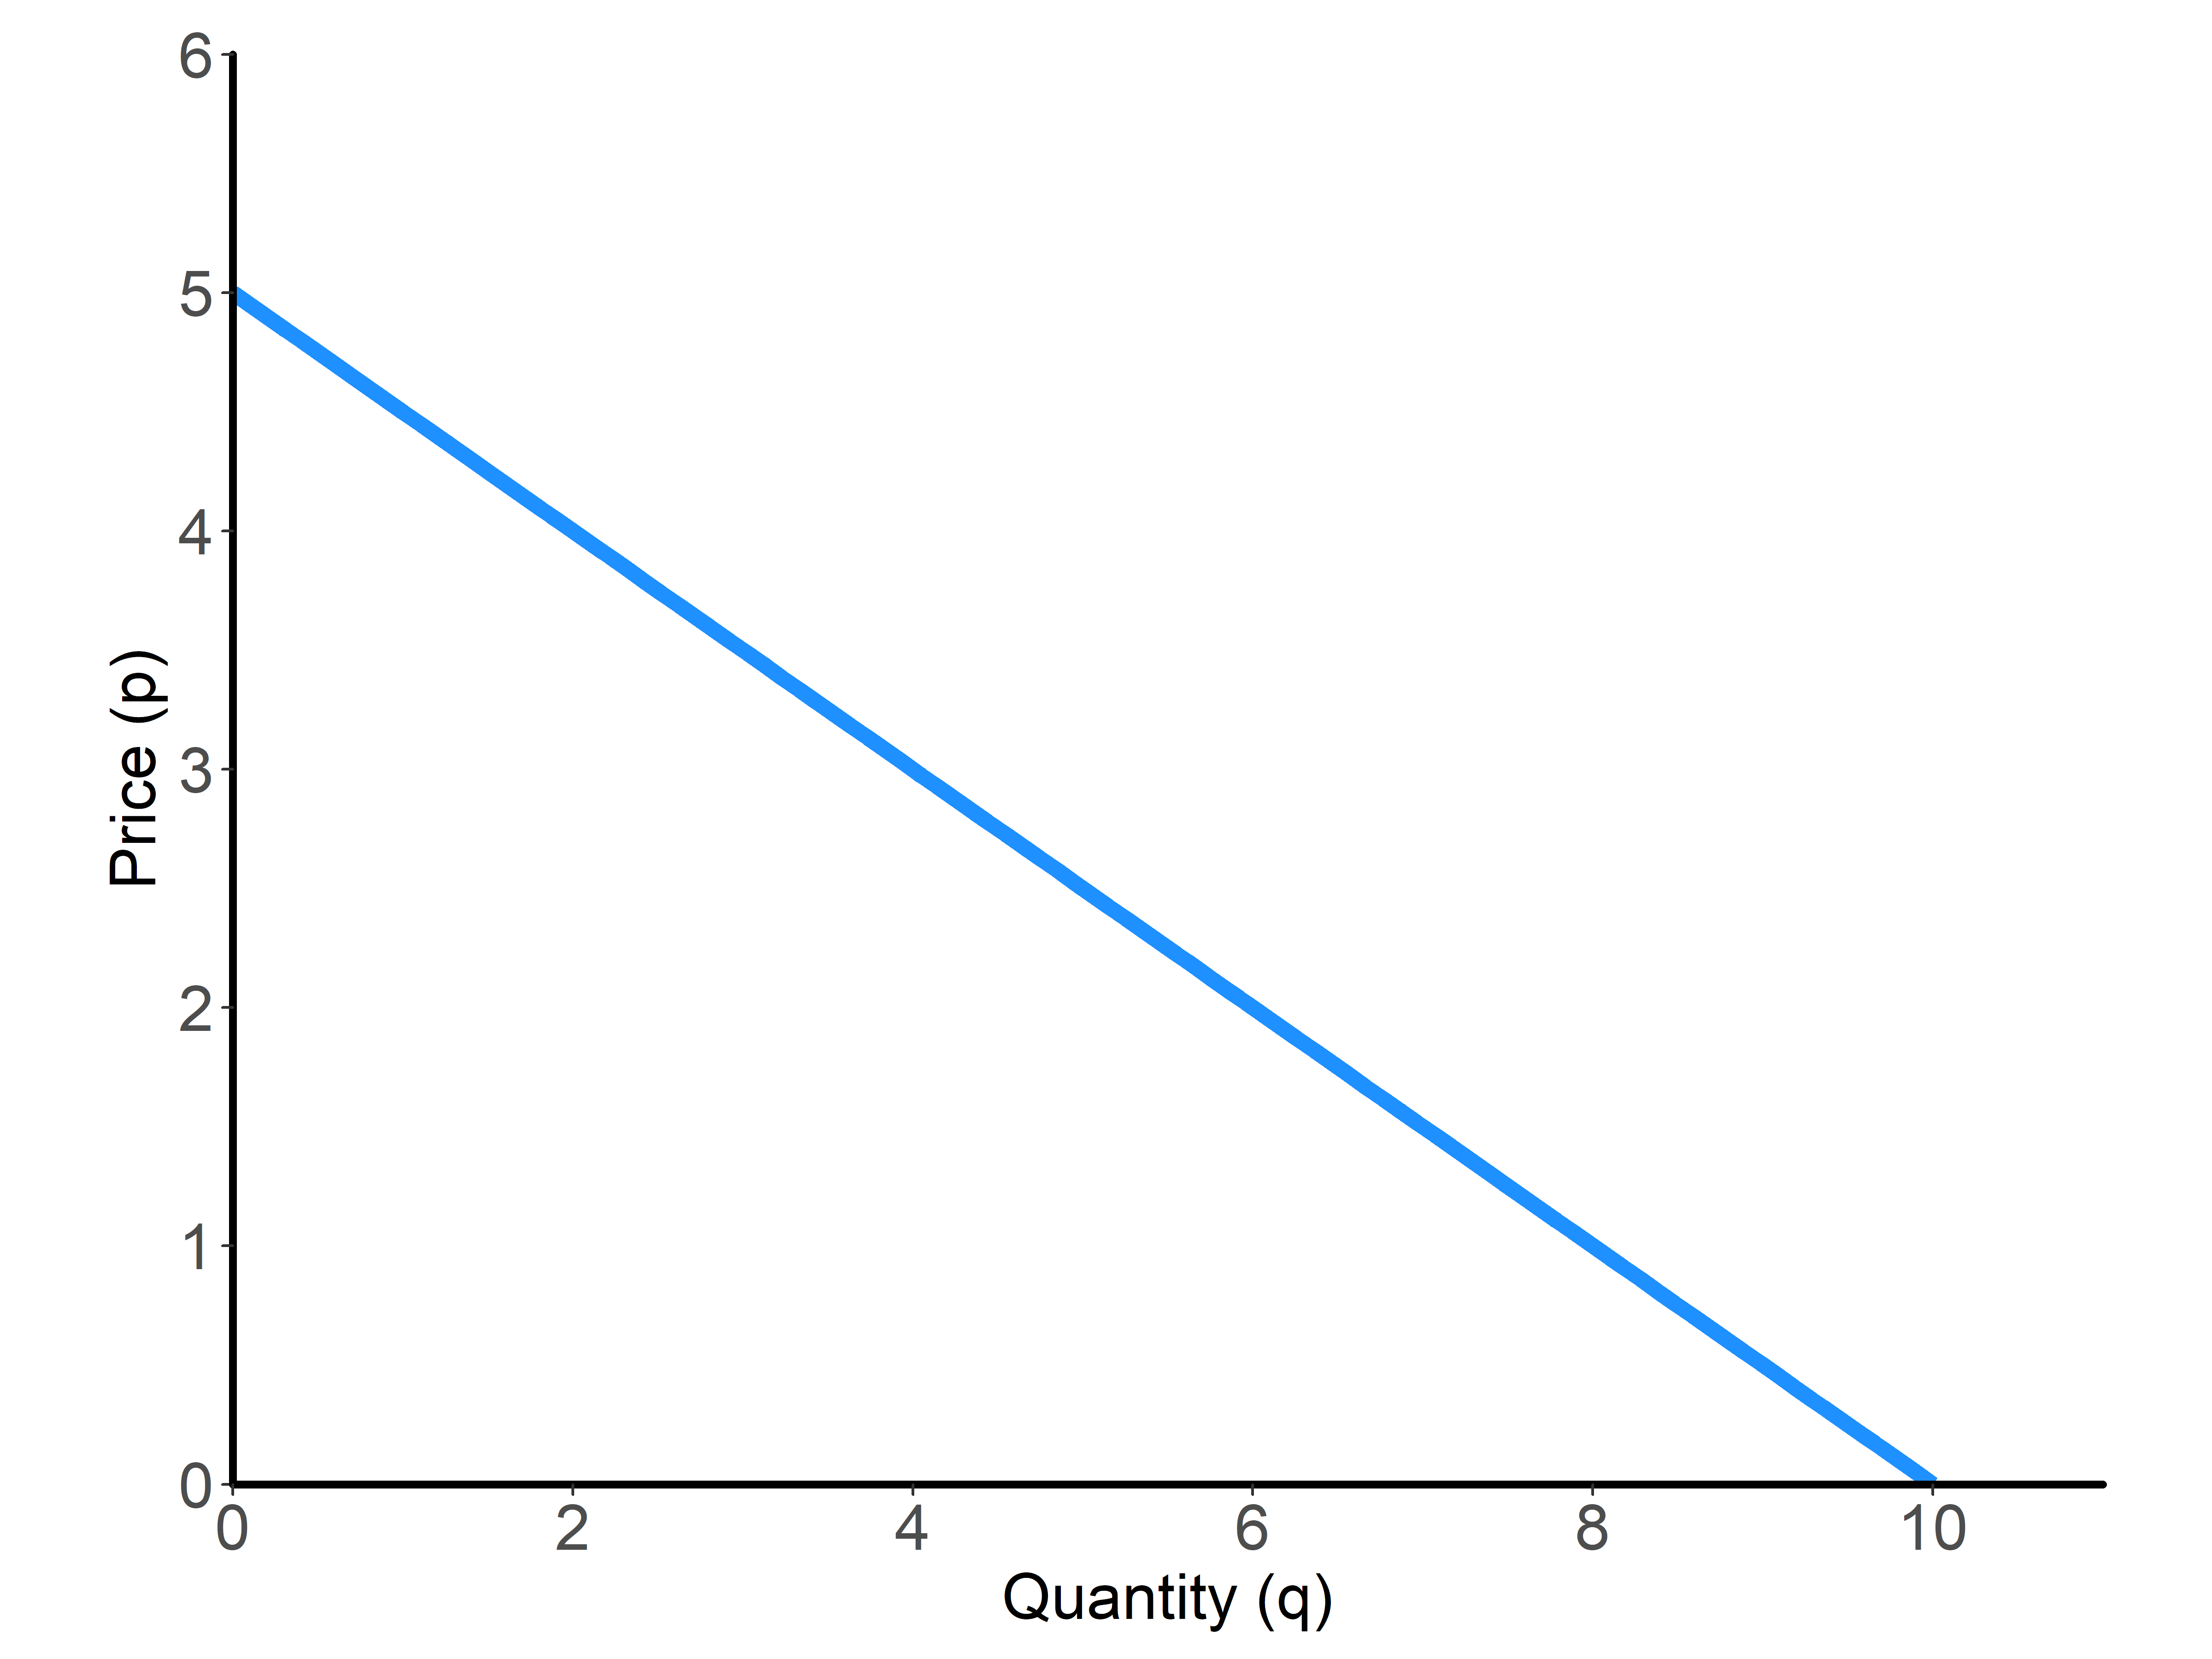
\includegraphics[width=0.65\textwidth]{../images/eq_1.png}
\end{center}

Where are things likely to go wrong? When you're in a time-crunch, if
you forget to check carefully what's given to you, you might end up
doing this:

\begin{center}
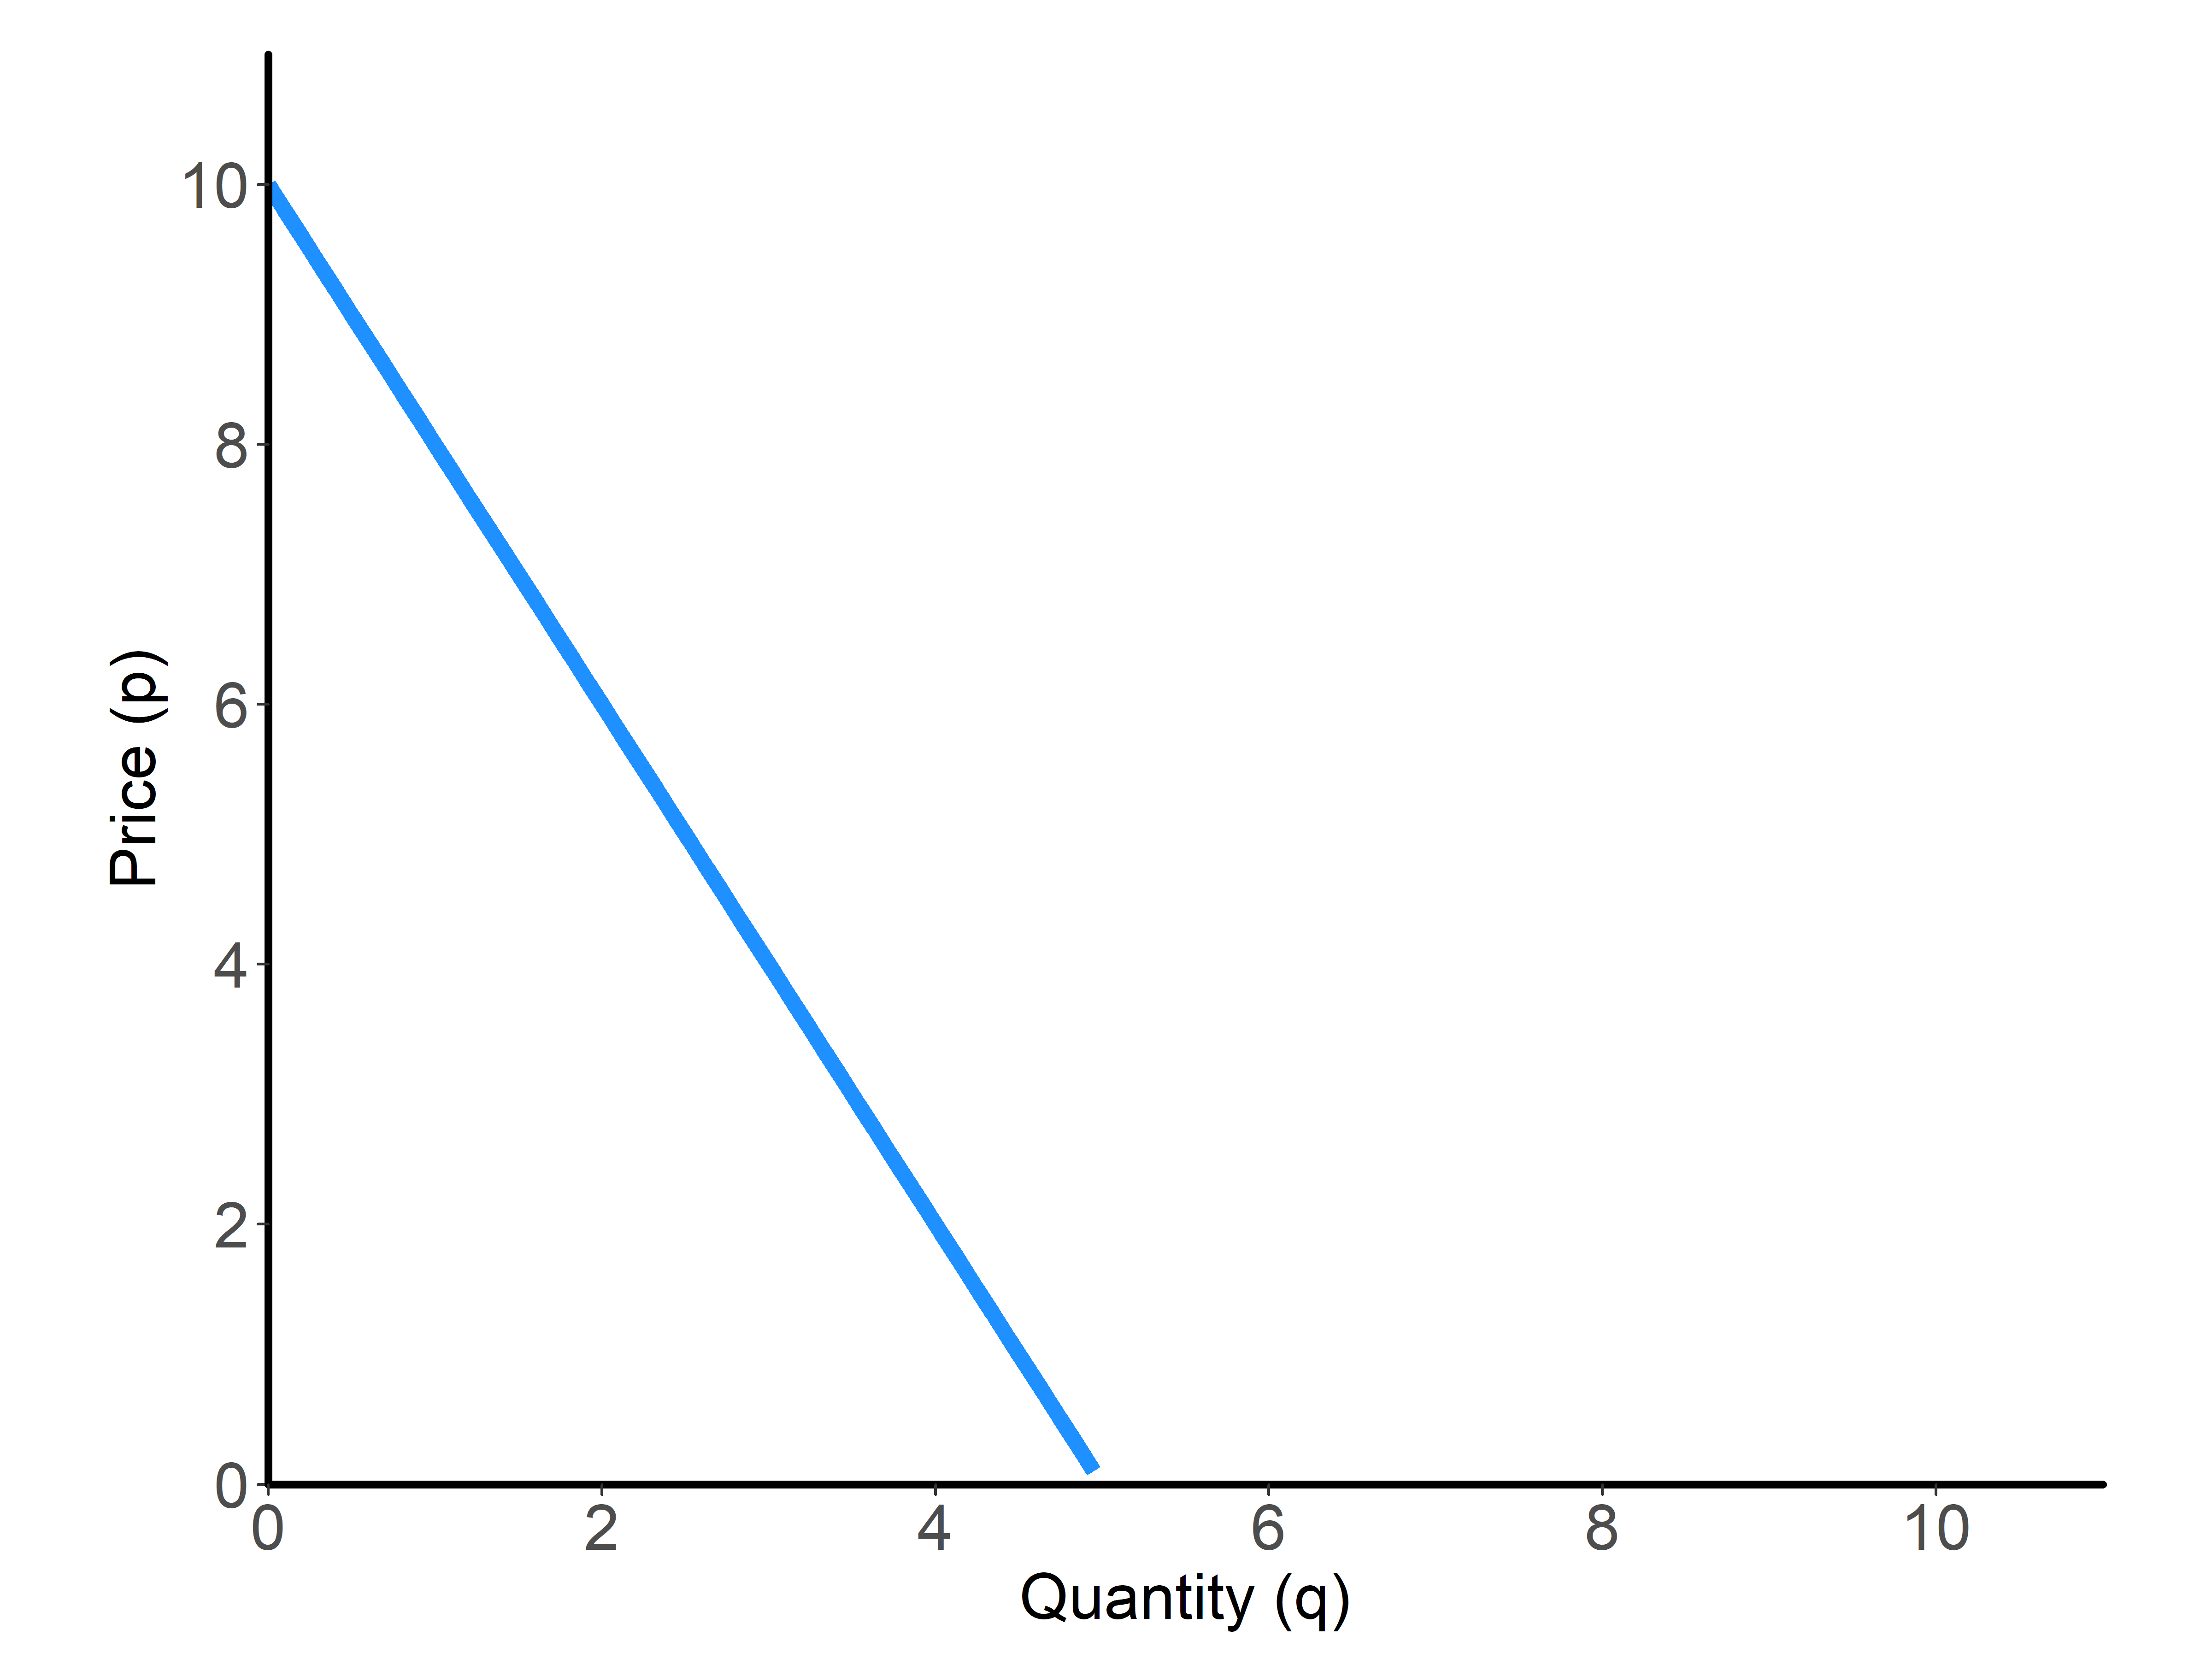
\includegraphics[width=0.65\textwidth]{../images/eq_wrong.png}
\end{center}

Can you spot what I've done wrong here?

A couple of useful error checks you can do at this point are to check
whether your inverse demand yields the same results as your original
demand function by substituting in a price and then seeing if I can get
the same price back at the end as follows:

\begin{align*}
  Q_d&=10-2p,\,\text{so it must be that at p=4, }Q_d=10-2(4)=2\\
  &\text{Let's see if this works in my inverse demand curve}\\
  p&=5-\frac{Q}{2}\,\text{, substituting in $Q_d=2$ yields:}\\
  p&=5-\frac{2}{2}=4\,\text{, which is where I started, so I know I've done it correctly.}
\end{align*}

Before you even get that far, it's often helpful to see if price is
decreasing in quantity. Since you know that the law of demand is such
that higher price means lower quantity demanded, it must also be the
case that higher quantity means lower willingness to pay, and so there
should be a negative sign on the term with \(Q\) in your function
determining \(p\).

\begin{enumerate}
\def\labelenumi{\arabic{enumi}.}
\setcounter{enumi}{1}
\tightlist
\item
  The next skill we're going to use is solving two equations with two
  unknowns (supply and demand solved for p and Q). So, let's use our
  previous example of \(Q_d=10-2p\) as demand, and use \(Q_s=3\,p\) as a
  simple supply curve. Now, to solve for equilibrium, we'll need a few
  steps.
\end{enumerate}

\begin{align*}
  Q_d&=10-2p,\,Q_s=3p\\
  10-2p&=3p\,\text{, after setting supply equal to demand}\\
  10&=3p+2p=5p\,\text{, after adding $2p$ to both sides of the equation}\\
  2&=p\,\text{, after dividing both sides of the equation by 5}\\
  &\text{and now we check our result and solve for quantity supplied AND demanded:}\\
  Q_s&=3p=3(2)=6\,\text{, after substituting the equilibrium price into the supply function}\\
  Q_d&=10-2p=10-2(2)=10-4=6\,\text{, after substituting the equilibrium price into the demand function.}\\
  &\text{This is a useful test because, if you don't get the same quantity, you've done it incorrectly.}
\end{align*}

Now, let's check this graphically. But, be careful! I need to convert my
supply curve to a function of price as well.

\begin{align*}
  Q&=3p\\
  \frac{Q}{3}&=p\,\text{, after dividing both sides by 3}\\
  p&=\frac{Q}{3}\,\text{, after rearranging terms}\\
\end{align*}

Here, again, we have an opportunity to check our work.

\begin{align*}
  Q&=3p,\,\text{so at $p=3$, $Q_s=9$}\\
  &\text{now, let's check that with our inverted supply function}\\
  p&=\frac{9}{3}=3\,\text{, which is where we started. Excellent.}\\
\end{align*}

Now, let's graph the supply curve on the same set of axes.

\begin{center}
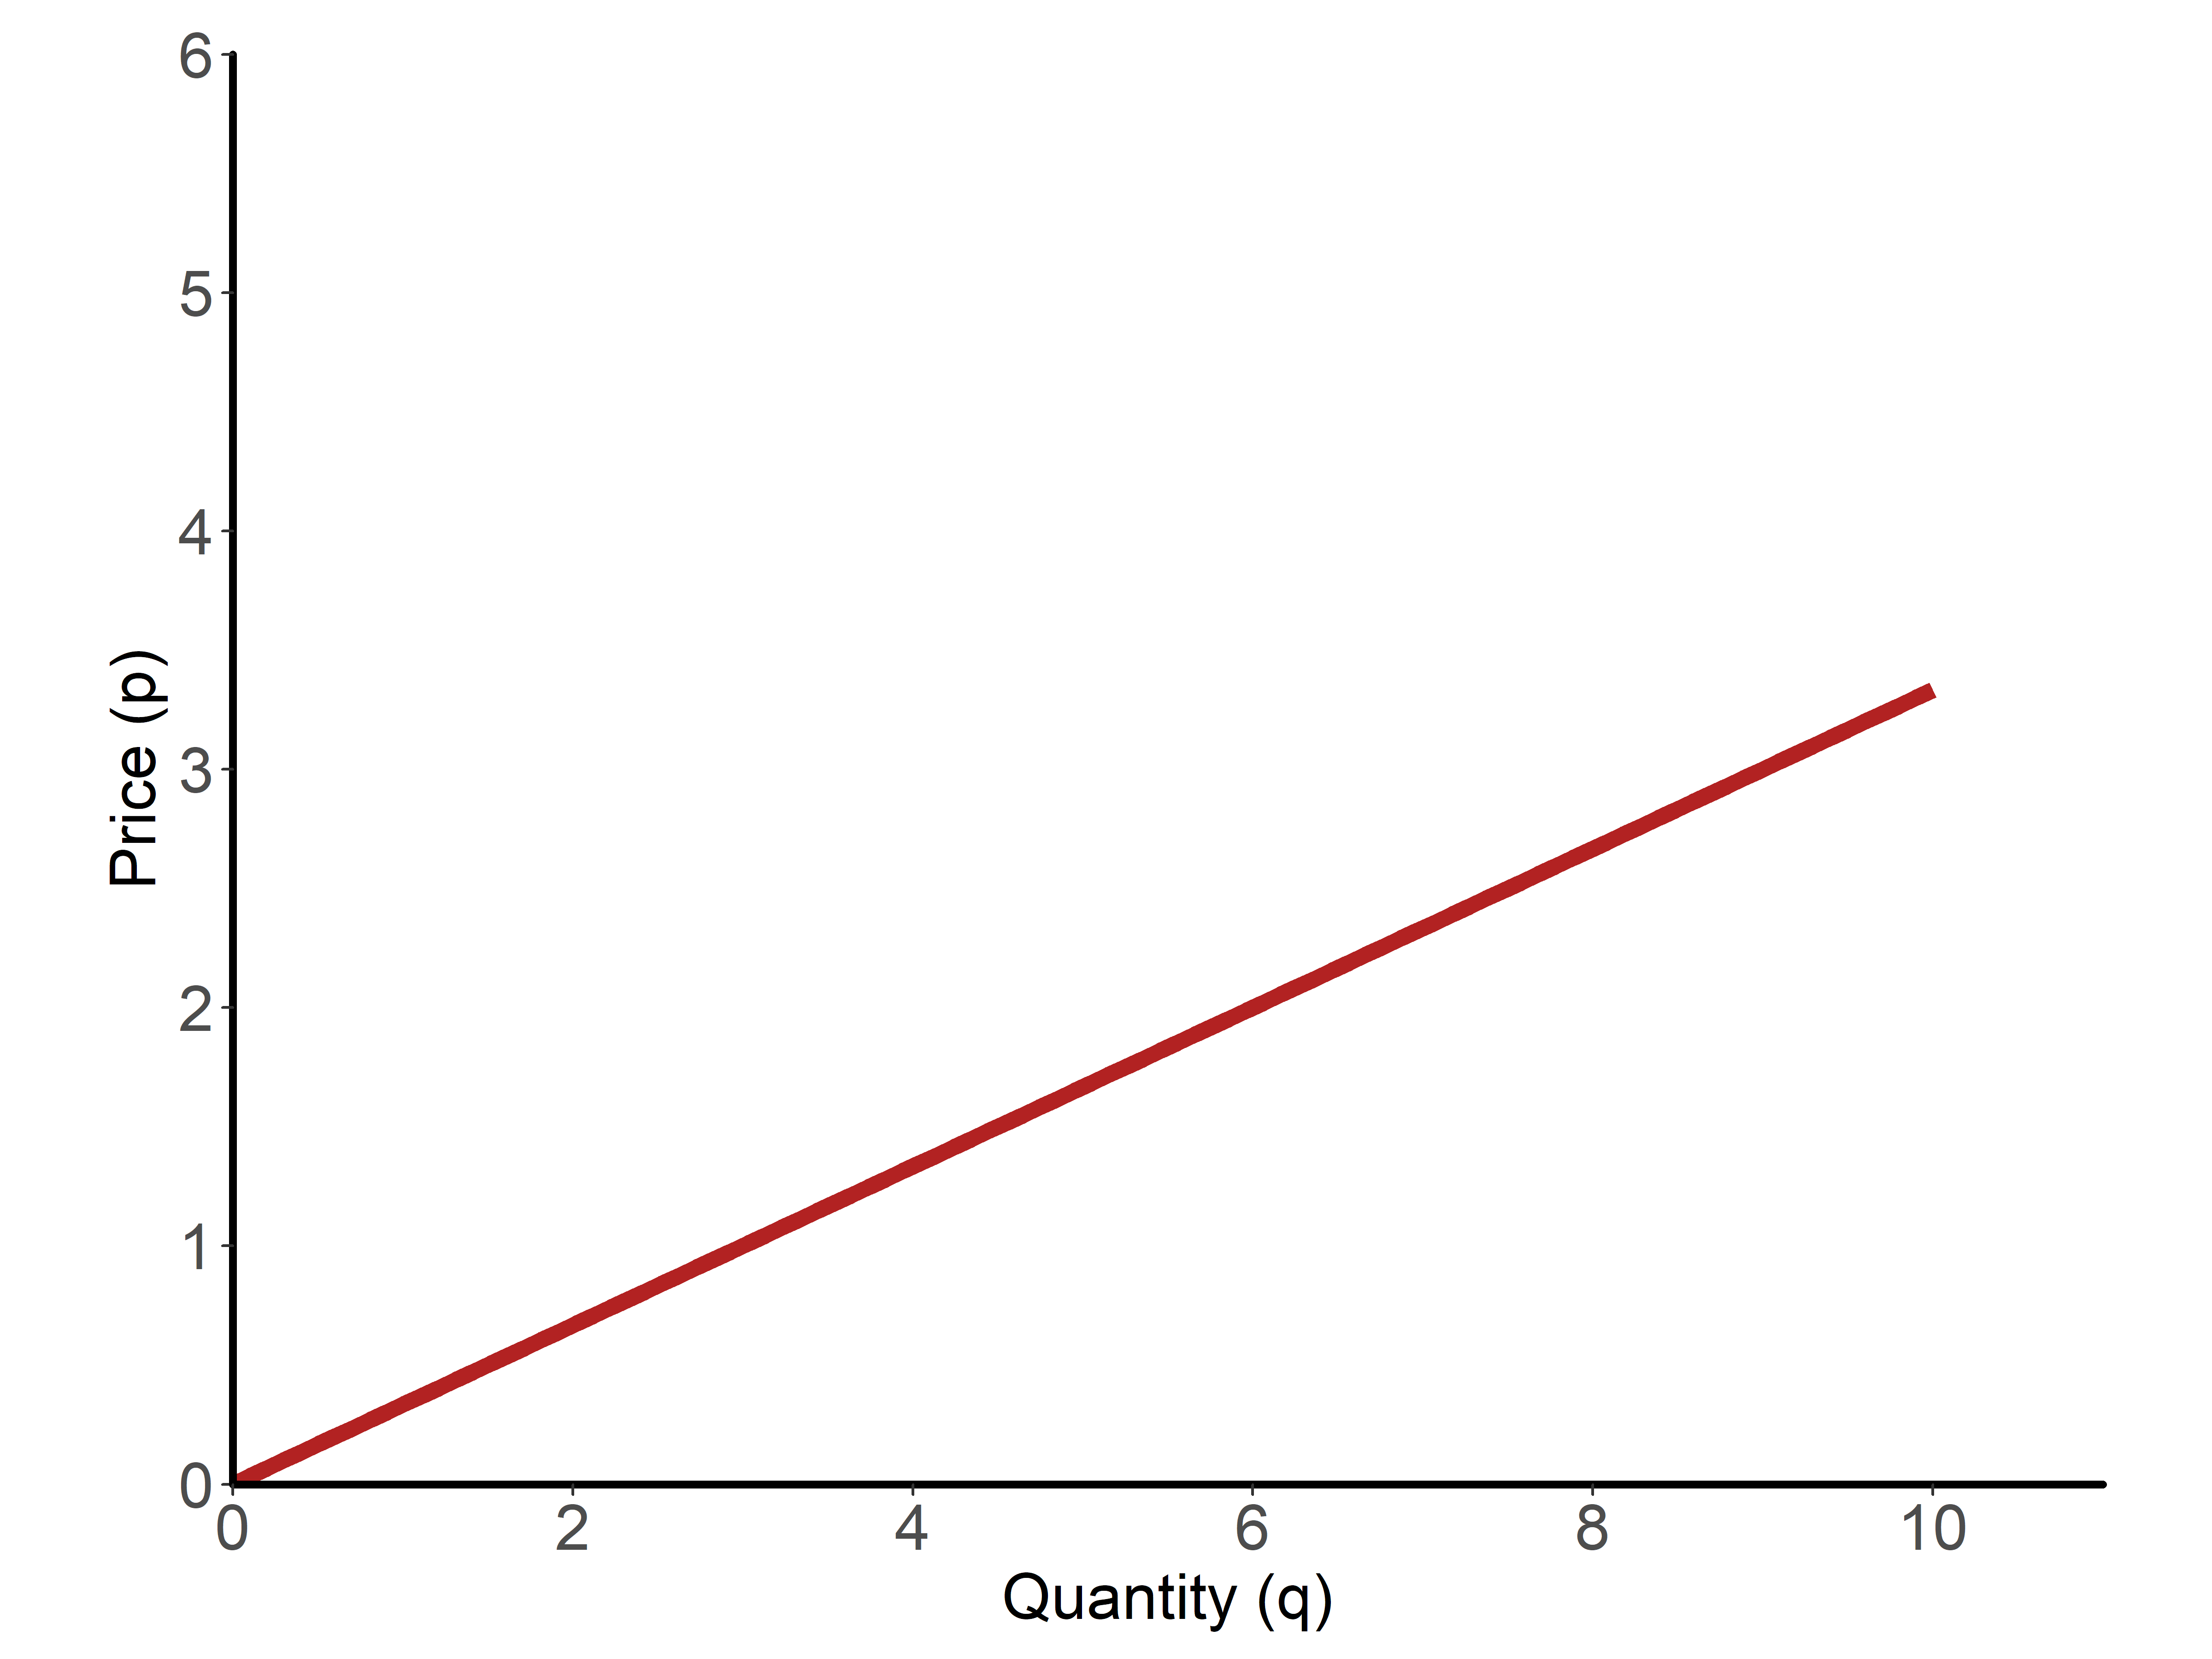
\includegraphics[width=0.65\textwidth]{../images/eg_supply.png}
\end{center}

When we add the supply and demand graphs on the same set of axes, the
equilibrium point is obvious, although you likely don't want to rely
just on your graphing skills to solve questions in the class!

\begin{center}
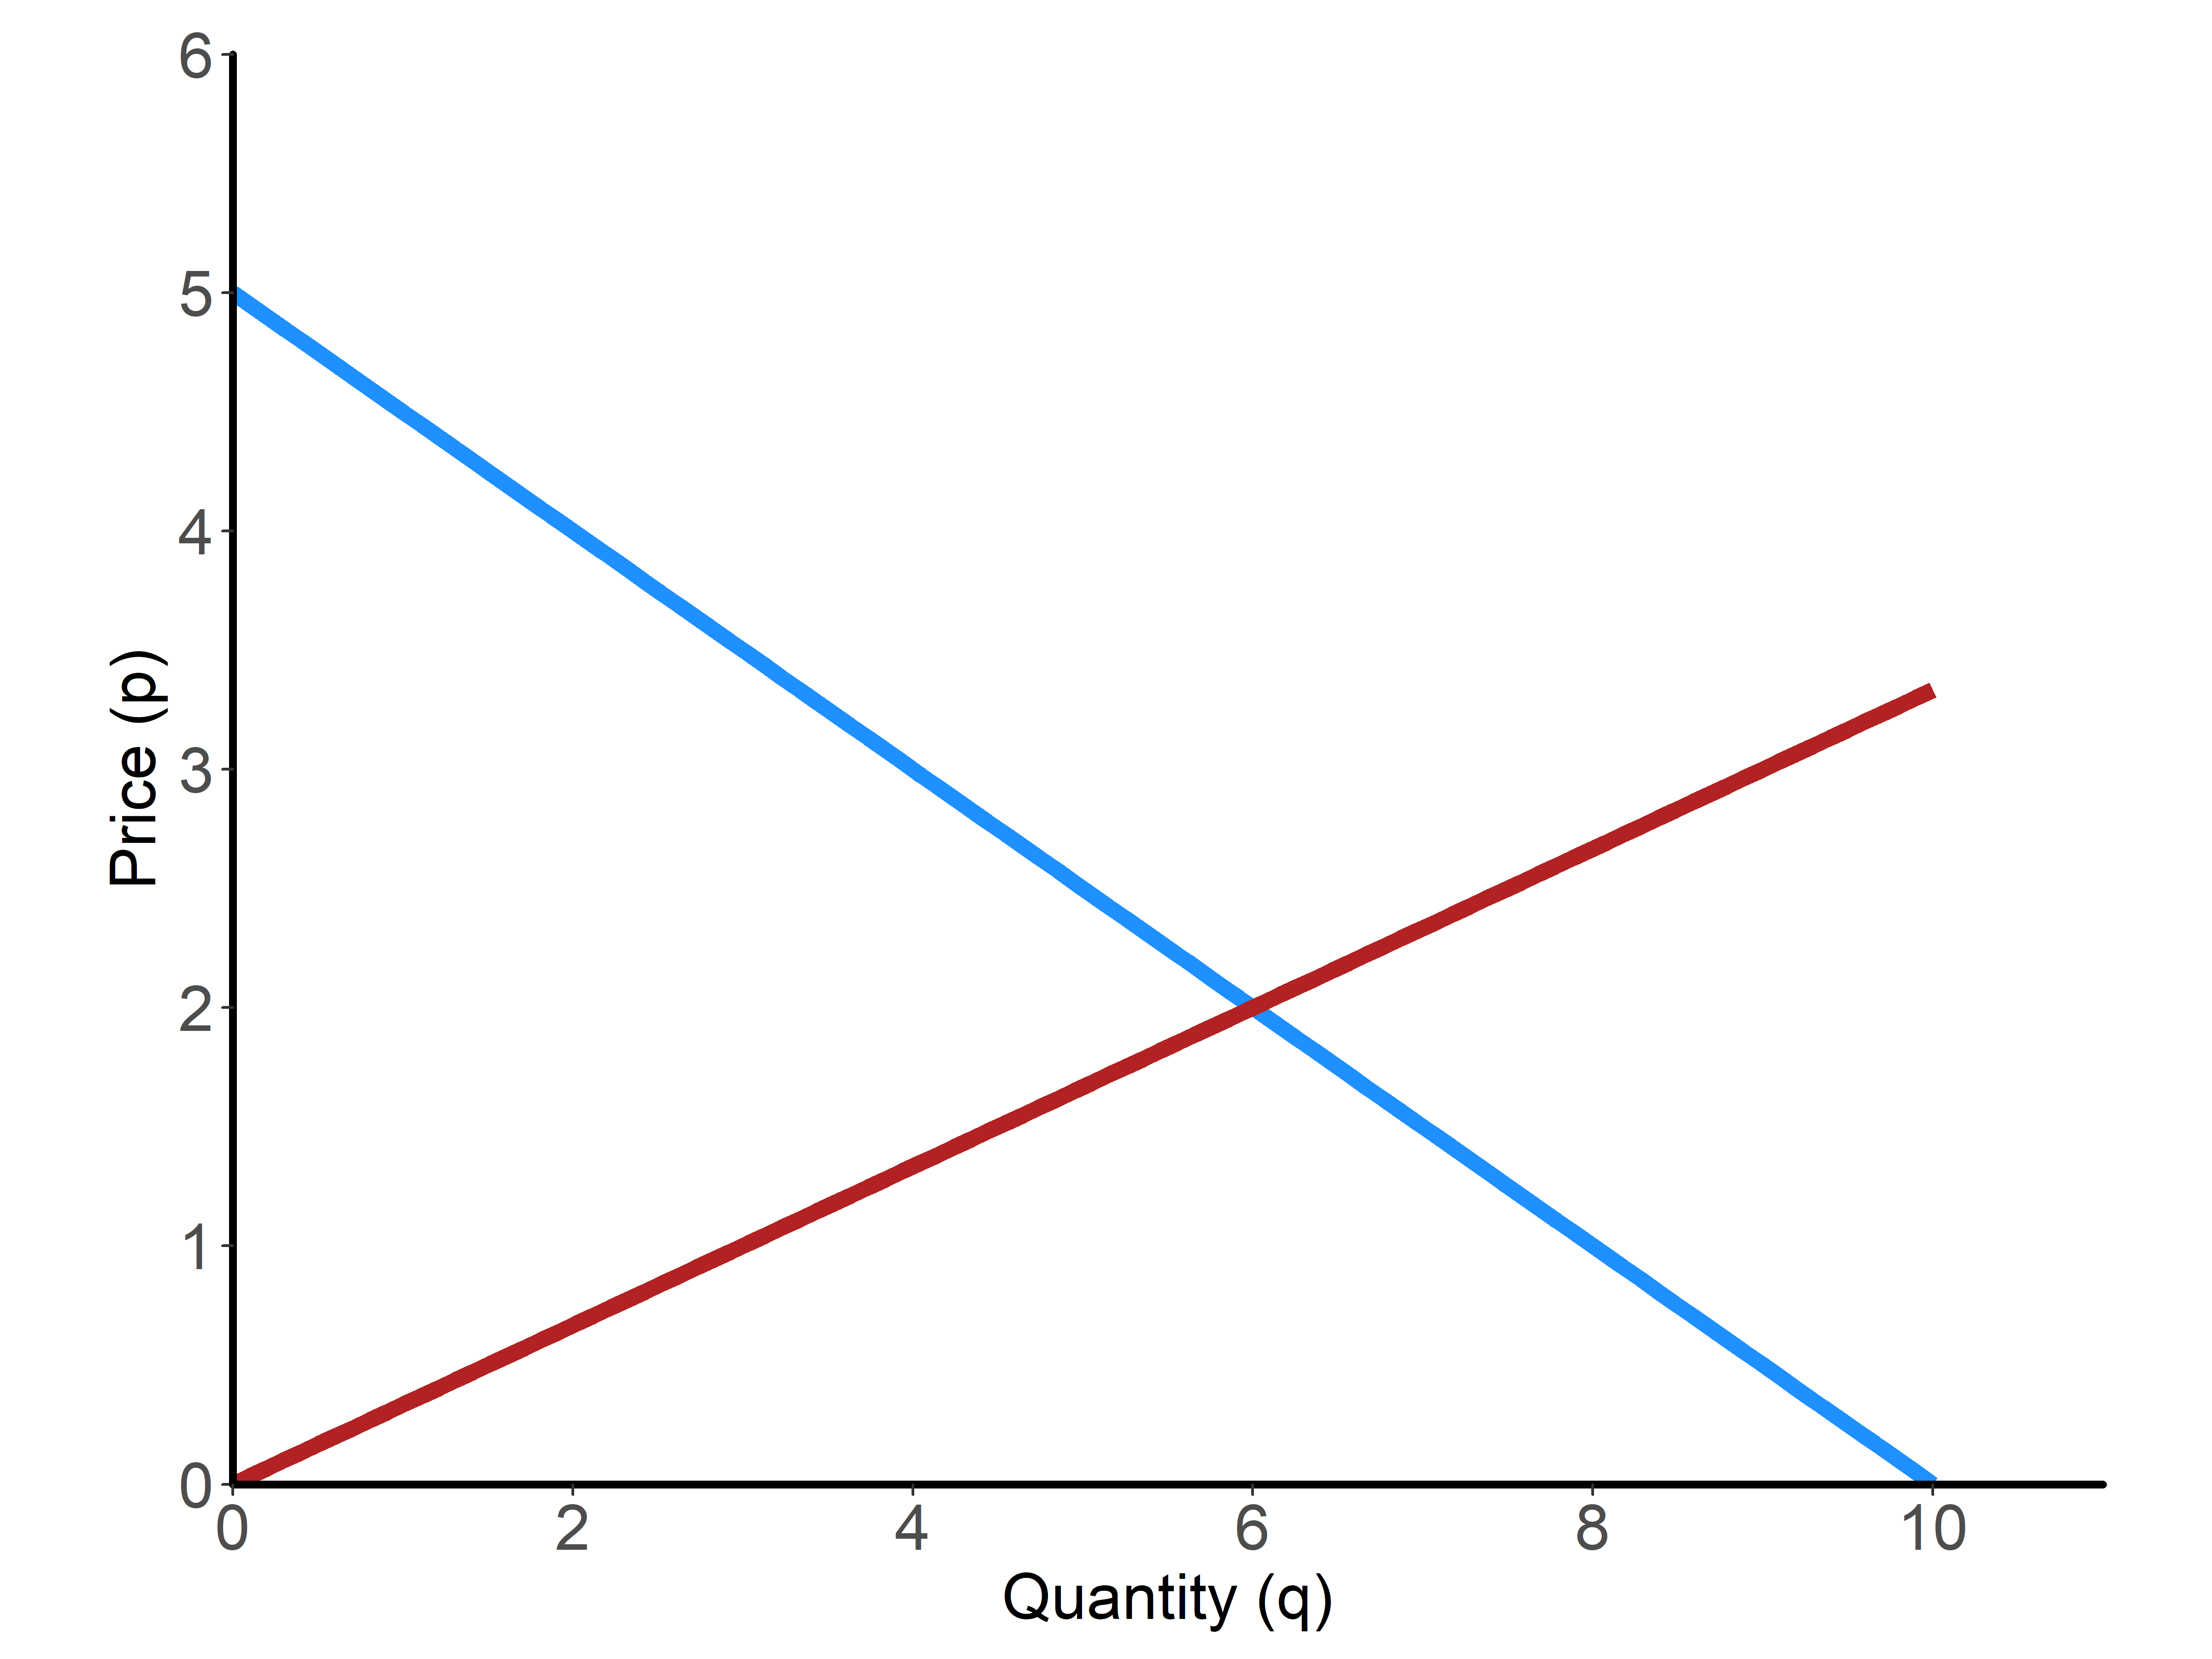
\includegraphics[width=0.65\textwidth]{../images/eg_both.png}
\end{center}

But, when we add some detail to the graphs, you can see the p=2, Q=6 is
indeed the equilibrium.

\begin{center}
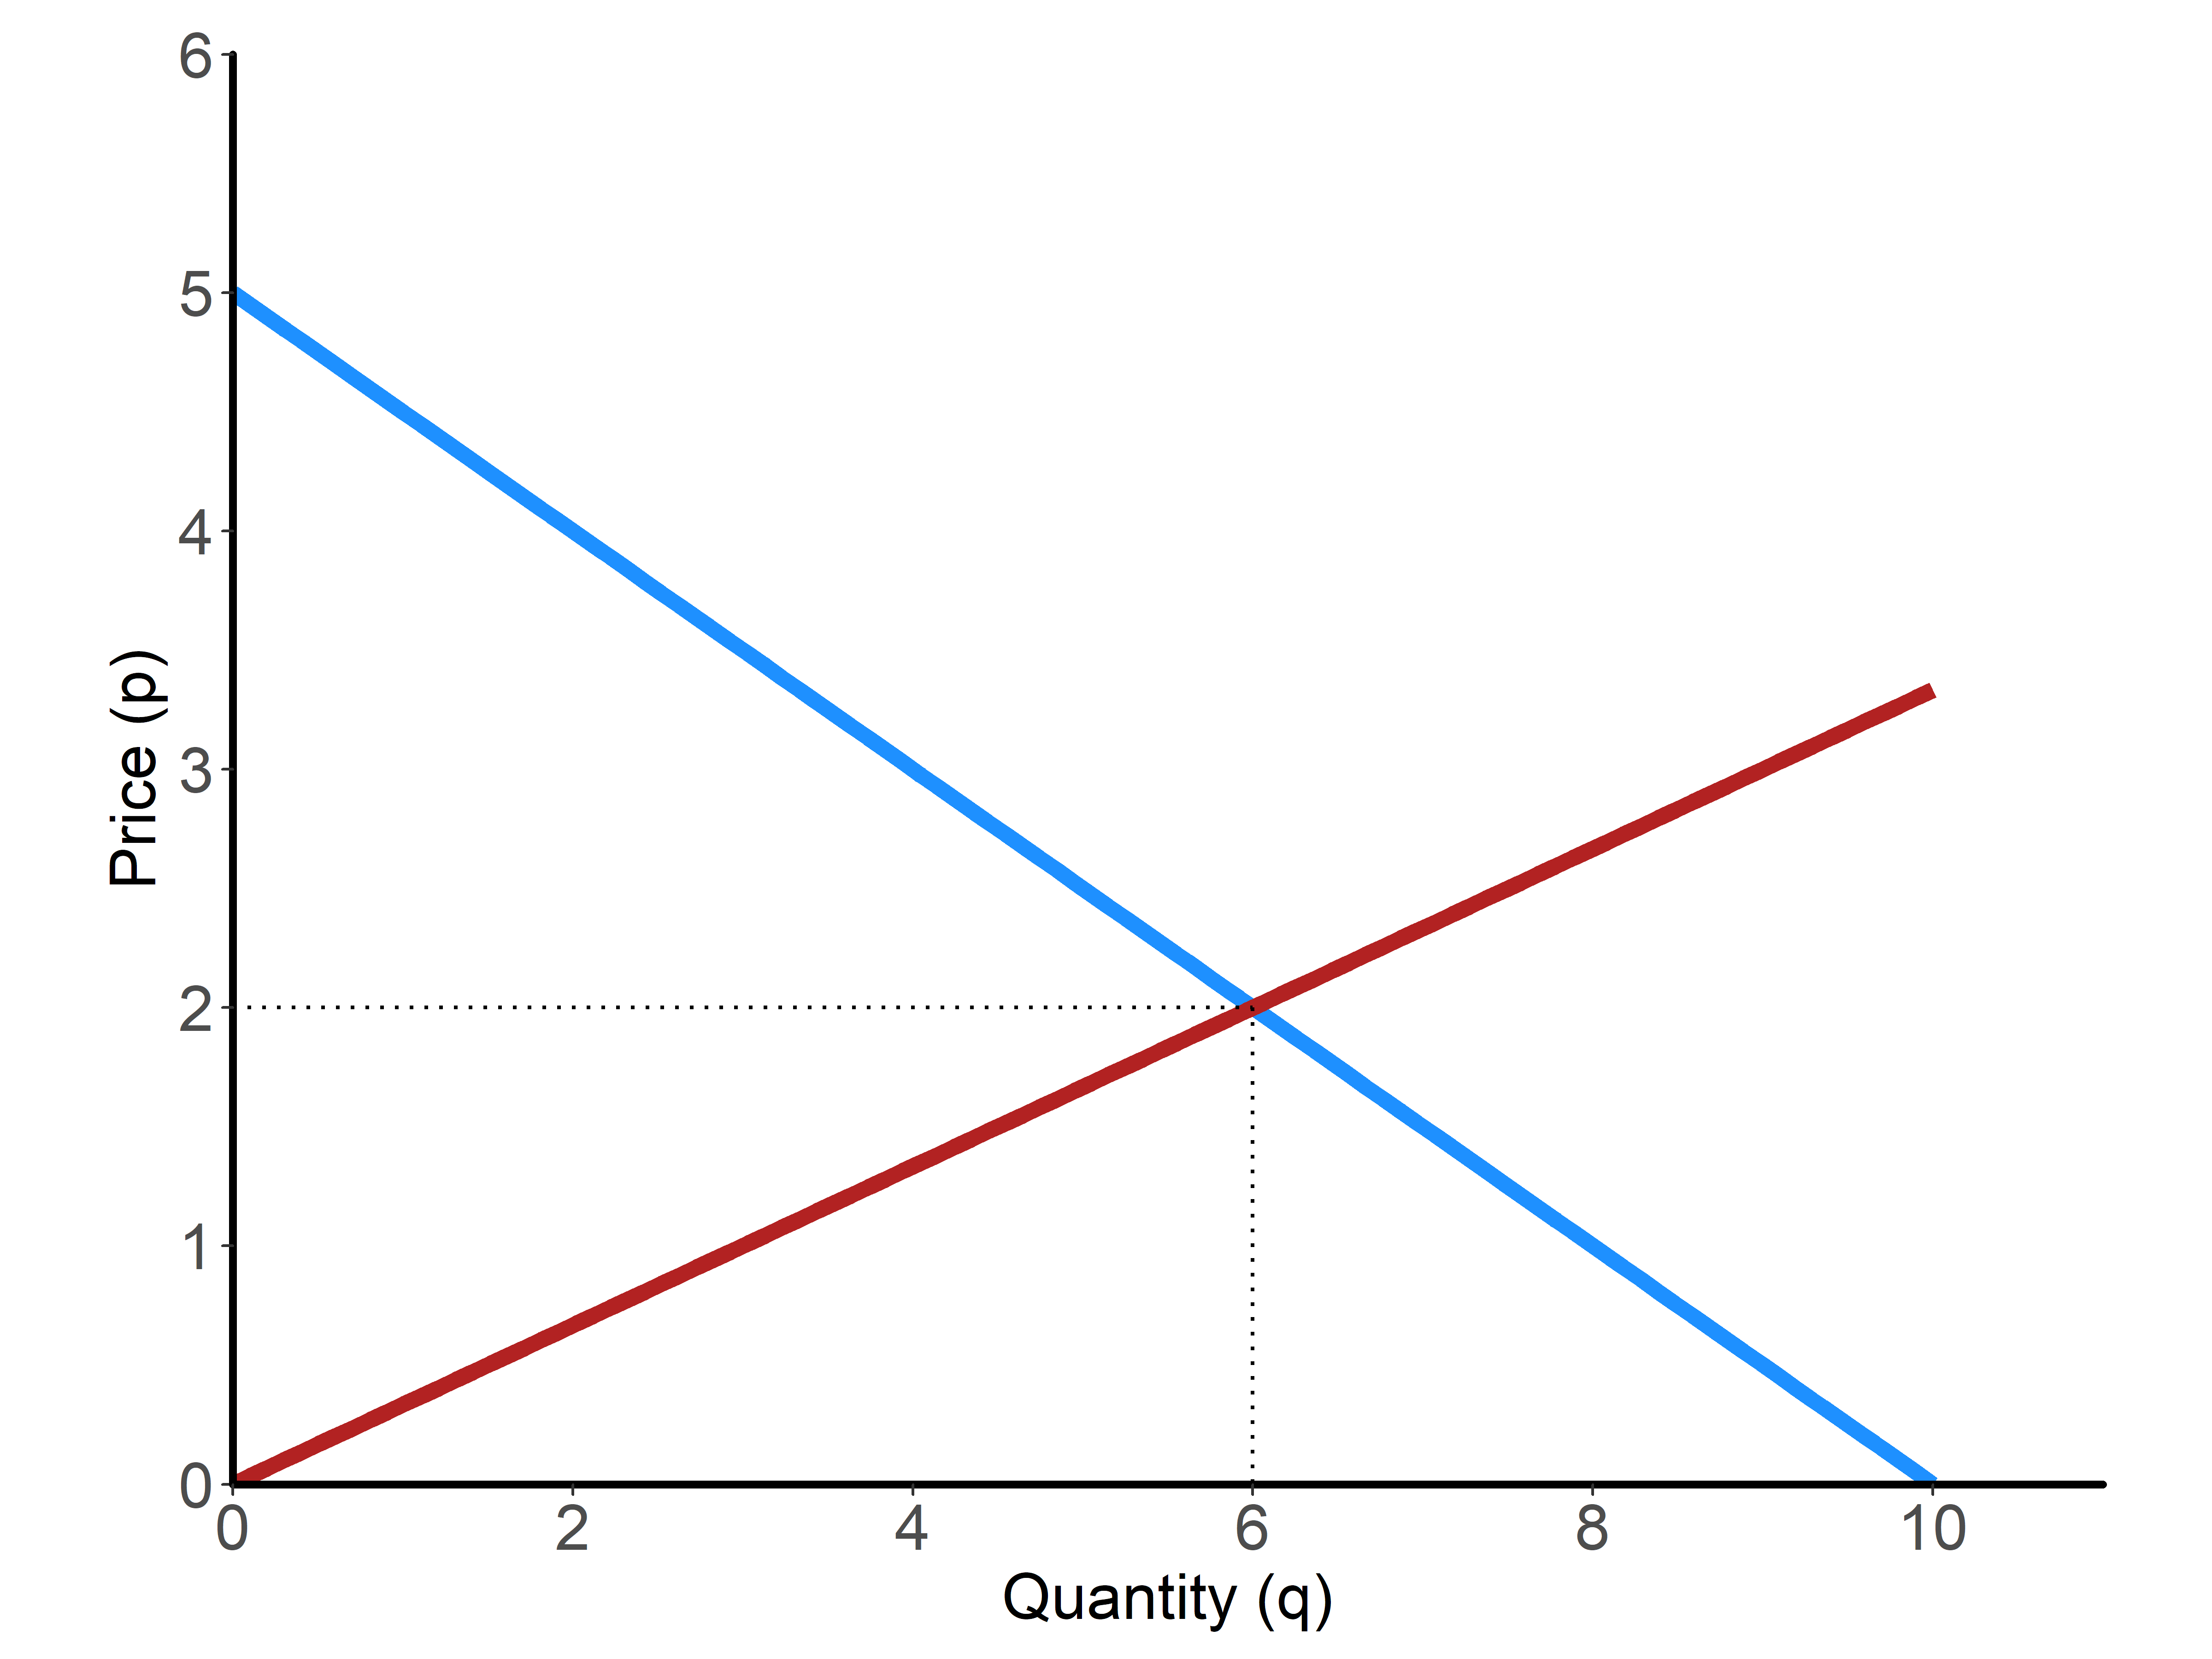
\includegraphics[width=0.65\textwidth]{../images/eg_equil.png}
\end{center}

Work through this step-by-step to see if you can replicate each step
without fail. If you have no issues with this, you're in good shape. The
steps are always the same, but the numbers might not always divide as
evenly as they do here.




\end{document}
